%Andrew Garcia's fork from Rob Agnese's Github repository (https://github.com/ragnese/beamer-theme-UF)
\documentclass{beamer}
\usepackage{float}
\usepackage{listings}
\usepackage{subcaption}
\usepackage{amsmath}
\usepackage{hyperref}
\usepackage{rotating}
%ARG Added: Landscape (widescreen) presentation 16:9
\usepackage{beamerthemesplit}
\usepackage[orientation=landscape,size=custom,width=16,height=9,scale=0.5,debug]{beamerposter} 

\hypersetup{colorlinks=true}
\usetheme{rob}
%\usetheme{Boadilla}
%\useinnertheme{circles}
%\useoutertheme{infolines}
%\usecolortheme{whale}


%\title[G4DMC]{Excessive Phonon Energy in G4DMC Events\\[1em]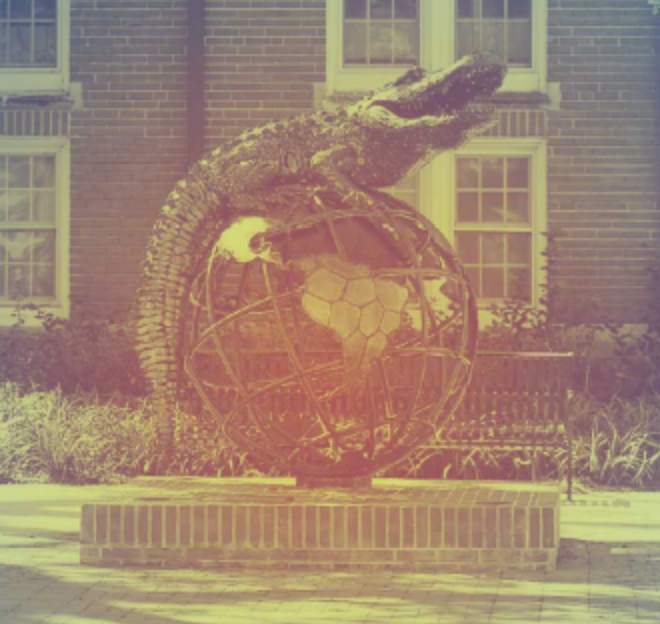
\includegraphics[width=3cm]{gator.png}}

\title[G4DMC]{Excessive Phonon Energy in G4DMC Events}
\titlegraphic{
\includegraphics[width=3.4cm]{UF_Monogram}}
\subtitle{\textbf{ \href{https://github.com/andrewrgarcia/beamer-theme-UF}{Andrew's fork} from \href{https://github.com/ragnese/beamer-theme-UF}{Rob Agnese's repository} }}

\author{Rob Agnese}
\institute{University of Florida}
\date{February 27, 2017}



\begin{document}

\begin{frame}[plain, noframenumbering]
    \titlepage{}
\end{frame}

\begin{frame}{The Problem}
    \vfill
    While debugging the track weighting discrepencies, I noticed that
    even without downsampling, we were getting too much energy out from a 
    simulation. \\

    For an electron recoil we should expect:
    \begin{equation}
        E_{phonon} = E_{recoil} + 4 \textrm{volt} \times 
        \textrm{floor}\left(\frac{E_{recoil}}{E_{pair}}\right)
    \end{equation}

    For the 1 keV event I tested, that should be $\sim$ 2.4 keV. G4DMC collected
    a total of $\sim$ 3.1 keV of phonon energy.
    \vfill
\end{frame}

\begin{frame}{Investigation}
    \vfill
    Some immediate consistency checks:
    \begin{itemize}
        \item Charge drift speeds still match data.
        \item Energy partitioner creates correct initial tracks (energies sum to $E_{recoil}$).
        \item Luke phonon emissions conserve energy on case-by-case basis.
    \end{itemize}
    \vfill
\end{frame}

\begin{frame}{Tests}
    \vfill
    We have checked several potential sources of error:
    \begin{itemize}
        \item Use uniform electric field instead of COMSOL field - \textbf{no change}.
        \item Turn off inter-valley scattering (known to be non-physical) - \textbf{no change}.
        \item Create only phonons - \textbf{Correct energy output}!
        \item Shoot exactly one charge carrier pair - \textbf{Excess still present}.
    \end{itemize}
    \vfill
\end{frame}

\begin{frame}{Places Left to Look}
    \vfill
    The bug must be in the charge physics. We've ruled out inter-valley scattering
    and Luke phonon emission. The drift curves also should rule out E-field
    acceleration bugs. There are three processes left:
    \begin{itemize}
        \item DriftBoundaryProcess - When a charge carrier is absorbed, releases
            its kinetic energy as phonons.
        \item DriftRecombinationProcess - When a charge carrier comes to rest
            in the crystal, it is killed and releases half of the gap energy
            as phonons.
        \item EnergyLimiter - When any particle is below its energy threshold,
            it is simply killed and deposits its kinetic energy as NIEL. This
            shouldn't be triggering ever for charge carriers as threshold = 0.
    \end{itemize}
    \vfill
\end{frame}

%ARG Added: Slides 5- 7 
%Credit -- Beamer Presentations: A Tutorial for Beginners (Part 2)—Lists, Columns, Pictures, Descriptions and Tables https://www.overleaf.com/learn/latex/Beamer_Presentations:_A_Tutorial_for_Beginners_(Part_2)%E2%80%94Lists,_Columns,_Pictures,_Descriptions_and_Tables

\begin{frame}
\frametitle{Using Columns}
\begin{columns}
\column{0.5\textwidth}
 Fusce arcu magna, faucibus non tellus ac, tincidunt accumsan eros. Fusce tempor sollicitudin feugiat. Phasellus mi quam, vehicula vitae ligula at, commodo tristique dolor. Nullam ligula sapien, ultricies ac sagittis ac, egestas ac ligula. Maecenas eu leo vel ligula rutrum lacinia ut in purus. Nulla a ipsum suscipit, egestas metus id, scelerisque nulla.
\column{0.5\textwidth}
Morbi sit amet nulla ex. In nec metus id urna consectetur bibendum. Pellentesque convallis arcu massa, id gravida nibh fermentum fermentum. Aenean nec luctus tellus, quis fringilla libero. Vestibulum ante ipsum primis in faucibus orci luctus et ultrices posuere cubilia curae; Vivamus sit amet purus et leo posuere lacinia ut eu est. 
\end{columns}
\end{frame}


\begin{frame}
\frametitle{Using Columns}
\begin{columns}
\column{0.5\textwidth}
Fusce aliquam magna sit amet erat ullamcorper laoreet. Mauris facilisis turpis malesuada, cursus felis sit amet, consectetur magna. Nam commodo ipsum ac ipsum semper, vitae malesuada purus tristique. Ut vitae mollis urna, a vestibulum metus. Nunc iaculis vehicula arcu, sed porta erat consequat non. Ut pulvinar diam sit amet dui suscipit suscipit. Nullam ultrices erat quis metus consectetur suscipit. Nam consectetur, purus at lacinia condimentum.
\column{0.5\textwidth}
\centering 
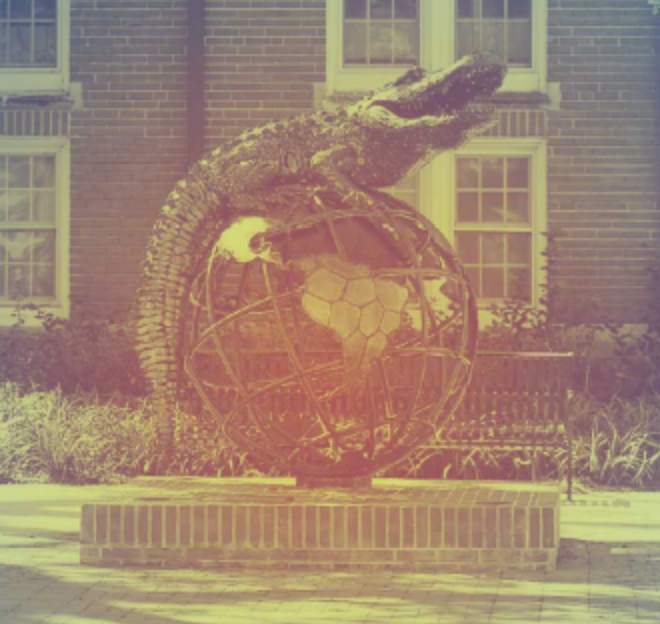
\includegraphics[width=3.5cm]{gator.png}
\end{columns}
\end{frame}



\begin{frame}
\frametitle{Pictures}
\begin{figure}
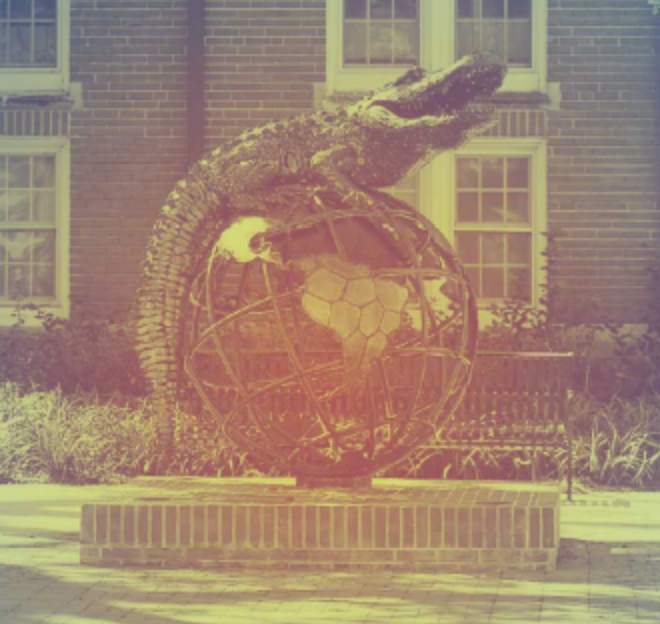
\includegraphics[scale=0.2]{gator.png}
\caption{scaled gator (0.2x)}
\end{figure}
Curabitur quis vehicula eros, mattis luctus libero. Mauris eget urna libero. Phasellus quis odio non odio tincidunt semper. Mauris hendrerit, lectus non gravida rutrum, ex ipsum egestas leo, non tincidunt magna.
\end{frame}

\begin{frame}{}
  \centering \Large
  \textbf{Thank You}
\end{frame}


\end{document}
